\documentclass[10pt,twocolumn]{article}
% Shared two-column preamble for the three research papers.
% Use with: \documentclass[10pt,twocolumn]{article}
% Then in main.tex: % Shared two-column preamble for the three research papers.
% Use with: \documentclass[10pt,twocolumn]{article}
% Then in main.tex: % Shared two-column preamble for the three research papers.
% Use with: \documentclass[10pt,twocolumn]{article}
% Then in main.tex: \input{../../shared/latex/twocolumn_preamble.tex}

\usepackage[margin=0.75in]{geometry}
\usepackage[utf8]{inputenc}
\usepackage[T1]{fontenc}
\usepackage{lmodern}
\usepackage{microtype}
\usepackage{amsmath,amssymb,amsthm}
\usepackage{graphicx}
\usepackage{booktabs}
\usepackage{caption}
\usepackage{subcaption}
\usepackage{hyperref}
\usepackage{url}
\usepackage{xcolor}
\usepackage{algorithm}
\usepackage{algorithmic}
\usepackage{multirow}
\usepackage{titlesec}
\usepackage{authblk}

\hypersetup{colorlinks=true,linkcolor=blue!50!black,citecolor=blue!50!black,urlcolor=blue!50!black}

\titleformat{\section}{\normalfont\large\bfseries}{\thesection}{0.6em}{}
\titleformat{\subsection}{\normalfont\bfseries}{\thesubsection}{0.5em}{}

\captionsetup{font=small,labelfont=bf,skip=4pt}
\setlength{\columnsep}{0.25in}
\setlength{\parskip}{2pt}

\newtheorem{theorem}{Theorem}
\newtheorem{proposition}[theorem]{Proposition}
\newtheorem{definition}[theorem]{Definition}


\usepackage[margin=0.75in]{geometry}
\usepackage[utf8]{inputenc}
\usepackage[T1]{fontenc}
\usepackage{lmodern}
\usepackage{microtype}
\usepackage{amsmath,amssymb,amsthm}
\usepackage{graphicx}
\usepackage{booktabs}
\usepackage{caption}
\usepackage{subcaption}
\usepackage{hyperref}
\usepackage{url}
\usepackage{xcolor}
\usepackage{algorithm}
\usepackage{algorithmic}
\usepackage{multirow}
\usepackage{titlesec}
\usepackage{authblk}

\hypersetup{colorlinks=true,linkcolor=blue!50!black,citecolor=blue!50!black,urlcolor=blue!50!black}

\titleformat{\section}{\normalfont\large\bfseries}{\thesection}{0.6em}{}
\titleformat{\subsection}{\normalfont\bfseries}{\thesubsection}{0.5em}{}

\captionsetup{font=small,labelfont=bf,skip=4pt}
\setlength{\columnsep}{0.25in}
\setlength{\parskip}{2pt}

\newtheorem{theorem}{Theorem}
\newtheorem{proposition}[theorem]{Proposition}
\newtheorem{definition}[theorem]{Definition}


\usepackage[margin=0.75in]{geometry}
\usepackage[utf8]{inputenc}
\usepackage[T1]{fontenc}
\usepackage{lmodern}
\usepackage{microtype}
\usepackage{amsmath,amssymb,amsthm}
\usepackage{graphicx}
\usepackage{booktabs}
\usepackage{caption}
\usepackage{subcaption}
\usepackage{hyperref}
\usepackage{url}
\usepackage{xcolor}
\usepackage{algorithm}
\usepackage{algorithmic}
\usepackage{multirow}
\usepackage{titlesec}
\usepackage{authblk}

\hypersetup{colorlinks=true,linkcolor=blue!50!black,citecolor=blue!50!black,urlcolor=blue!50!black}

\titleformat{\section}{\normalfont\large\bfseries}{\thesection}{0.6em}{}
\titleformat{\subsection}{\normalfont\bfseries}{\thesubsection}{0.5em}{}

\captionsetup{font=small,labelfont=bf,skip=4pt}
\setlength{\columnsep}{0.25in}
\setlength{\parskip}{2pt}

\newtheorem{theorem}{Theorem}
\newtheorem{proposition}[theorem]{Proposition}
\newtheorem{definition}[theorem]{Definition}

% Auto-generated by src/figures/plot_corridor.py -- do not edit.
\newcommand{\InvLengthKm}{10.0}
\newcommand{\InvApproaches}{226}
\newcommand{\InvApproachesNoService}{99}
\newcommand{\InvServiceApproaches}{110}
\newcommand{\InvAccessesNoService}{97}
\newcommand{\InvFeederLanes}{264}
\newcommand{\InvFeederLanesNoService}{133}
\newcommand{\InvRetornos}{17}
\newcommand{\InvLanesMajor}{30}
\newcommand{\InvNMajor}{20}
\newcommand{\InvLanesTertiary}{46}
\newcommand{\InvNTertiary}{26}
\newcommand{\InvLanesMinor}{57}
\newcommand{\InvNMinor}{53}
\newcommand{\InvLanesService}{110}
\newcommand{\InvNService}{110}
\newcommand{\InvLanesRetorno}{21}
\newcommand{\InvNRetorno}{17}
\newcommand{\InvMainlineLanes}{5}
\newcommand{\InvExpressLanes}{3}
\newcommand{\InvMainlineMin}{2}
\newcommand{\InvMainlineMax}{7}
\newcommand{\InvLaneRatio}{26}
\newcommand{\InvLaneRatioNoService}{13}
\newcommand{\InvTaggedPct}{28}
\newcommand{\InvCorridorTaggedPct}{100}
\newcommand{\InvInternalLinks}{52}
\newcommand{\InvSignalsOSM}{4}
\newcommand{\InvSignalsWB}{7}
\newcommand{\InvSignalsEB}{8}
\newcommand{\InvJunctions}{11}
\newcommand{\InvCrossing}{33}
\newcommand{\InvTerminal}{193}
\newcommand{\InvFetched}{2026-10-12}
\newcommand{\LLMAccLo}{80}
\newcommand{\LLMAccHi}{100}
\newcommand{\LLMLanesLo}{130}
\newcommand{\LLMLanesHi}{160}
\newcommand{\LLMMainLo}{5}
\newcommand{\LLMMainHi}{6}
\newcommand{\ThQMajor}{800}
\newcommand{\ThQTertiary}{450}
\newcommand{\ThQMinor}{100}
\newcommand{\ThQService}{25}
\newcommand{\ThUp}{3500}
\newcommand{\ThG}{0.55}
\newcommand{\ThTurnCross}{0.30}
\newcommand{\ThFriction}{1.5}
\newcommand{\ThFifo}{0.5}
\newcommand{\ThDrop}{8}
\newcommand{\AnaWBMaxRho}{0.88}
\newcommand{\AnaWBBottleneckKm}{4.6}
\newcommand{\AnaWBSideVph}{14,900}
\newcommand{\AnaWBSideLanes}{121}
\newcommand{\AnaWBPerLane}{123}
\newcommand{\AnaWBPerLanePct}{6}
\newcommand{\AnaWBSatVph}{230,000}
\newcommand{\AnaWBPeakFlow}{6,700}
\newcommand{\PeakWBDelay}{0}
\newcommand{\PeakWBPerVeh}{-0.0}
\newcommand{\PeakWBQueueKm}{0.0}
\newcommand{\PeakWBHeadKm}{--}
\newcommand{\PeakWBFluid}{0}
\newcommand{\PeakWBFifoLo}{-0}
\newcommand{\PeakWBFifoHi}{-0}
\newcommand{\GapWBDelay}{-0}
\newcommand{\GapWBMaxRho}{0.76}
\newcommand{\GapWBHeadKm}{0.0}
\newcommand{\GridWBOnset}{1.2}
\newcommand{\GridWBTopPerVeh}{7}
\newcommand{\GridWBTopScale}{1.4}
\newcommand{\AnaEBMaxRho}{1.36}
\newcommand{\AnaEBBottleneckKm}{4.5}
\newcommand{\AnaEBSideVph}{21,600}
\newcommand{\AnaEBSideLanes}{143}
\newcommand{\AnaEBPerLane}{151}
\newcommand{\AnaEBPerLanePct}{8}
\newcommand{\AnaEBSatVph}{272,000}
\newcommand{\AnaEBPeakFlow}{7,800}
\newcommand{\PeakEBDelay}{15,240}
\newcommand{\PeakEBPerVeh}{10.0}
\newcommand{\PeakEBQueueKm}{6.0}
\newcommand{\PeakEBHeadKm}{4.4}
\newcommand{\PeakEBFluid}{10,160}
\newcommand{\PeakEBFifoLo}{4,170}
\newcommand{\PeakEBFifoHi}{61,510}
\newcommand{\GapEBDelay}{2,940}
\newcommand{\GapEBMaxRho}{1.03}
\newcommand{\GapEBHeadKm}{2.3}
\newcommand{\GridEBOnset}{0.8}
\newcommand{\GridEBTopPerVeh}{36}
\newcommand{\GridEBTopScale}{1.4}
\newcommand{\ValErr}{3.2}
\newcommand{\ValErrMax}{20}
\newcommand{\ValSigErr}{8}
\newcommand{\ValCtmFluidErr}{0.00}
\newcommand{\ValN}{30}
\newcommand{\McDraws}{48}
\newcommand{\McRuns}{96}
\newcommand{\McCongested}{59}
\newcommand{\McCongestedPct}{61}
\newcommand{\McHitLR}{0}
\newcommand{\McGapHitLR}{70}
\newcommand{\McEqHitLR}{nan}
\newcommand{\McSpLR}{0.07}
\newcommand{\McHitLRC}{81}
\newcommand{\McGapHitLRC}{0}
\newcommand{\McEqHitLRC}{nan}
\newcommand{\McSpLRC}{0.17}
\newcommand{\McHitFC}{0}
\newcommand{\McGapHitFC}{0}
\newcommand{\McEqHitFC}{nan}
\newcommand{\McSpFC}{-0.14}
\newcommand{\McHitCap}{100}
\newcommand{\McGapHitCap}{0}
\newcommand{\McEqHitCap}{nan}
\newcommand{\McSpCap}{0.45}
\newcommand{\McHitRho}{100}
\newcommand{\McGapHitRho}{52}
\newcommand{\McEqHitRho}{nan}
\newcommand{\McSpRho}{0.43}
\newcommand{\McGapCongested}{23}
\newcommand{\McEqCongested}{0}
\newcommand{\McAcc}{100}
\newcommand{\McAuc}{1.00}
\newcommand{\McDelayMedian}{1,570}
\newcommand{\McGapDelayMedian}{0}
\newcommand{\McFalsified}{no}
\newcommand{\McWhereWB}{100}
\newcommand{\McWhereEB}{100}
\newcommand{\ItvN}{26}
\newcommand{\ItvMetMedian}{+15}
\newcommand{\ItvMetBetter}{35}
\newcommand{\ItvMetWorse}{65}
\newcommand{\ItvMetBaseEB}{-5}
\newcommand{\ItvConMedian}{-4}
\newcommand{\ItvConBetter}{77}
\newcommand{\ItvConWorse}{4}
\newcommand{\ItvConBaseEB}{-9}
\newcommand{\ItvLaneMedian}{-37}
\newcommand{\ItvLaneBetter}{100}
\newcommand{\ItvLaneWorse}{0}
\newcommand{\ItvLaneBaseEB}{-37}
\newcommand{\ItvRetMedian}{-0.3}
\newcommand{\ItvRetBetter}{8}
\newcommand{\ItvRetWorse}{8}
\newcommand{\ItvRetBaseEB}{-0}
\newcommand{\FcName}{Av. Alfonso Reyes}
\newcommand{\FcDir}{WB}
\newcommand{\FcLo}{570}
\newcommand{\FcHi}{770}
\newcommand{\FcKm}{3.87}
\newcommand{\FcAssumed}{2,100}
\newcommand{\NcWBMaxRho}{1.04}
\newcommand{\NcWBDelay}{1,360}
\newcommand{\NcWBQueueKm}{2.1}
\newcommand{\NcEBMaxRho}{1.36}
\newcommand{\NcEBDelay}{15,240}
\newcommand{\NcEBQueueKm}{6.0}
\newcommand{\McCongWB}{23}
\newcommand{\McCongEB}{100}
\newcommand{\DayWBMaxRho}{0.88}
\newcommand{\DayWBRhoSeven}{0.88}
\newcommand{\DayWBQueueKm}{0.0}
\newcommand{\DayWBCongH}{0.0}
\newcommand{\DayWBDelay}{0}
\newcommand{\DayWBCap}{5,360}
\newcommand{\DayWBStart}{--}
\newcommand{\DayWBEnd}{--}
\newcommand{\DayWBClears}{never forms}
\newcommand{\DayWBPQueue}{12}
\newcommand{\DayWBCongHMed}{0.0}
\newcommand{\DayEBMaxRho}{1.36}
\newcommand{\DayEBRhoSeven}{0.52}
\newcommand{\DayEBQueueKm}{6.0}
\newcommand{\DayEBCongH}{4.3}
\newcommand{\DayEBDelay}{17,060}
\newcommand{\DayEBCap}{5,530}
\newcommand{\DayEBStart}{15:44}
\newcommand{\DayEBEnd}{19:59}
\newcommand{\DayEBClears}{is still there at 20:00, the end of the simulated day}
\newcommand{\DayEBPQueue}{100}
\newcommand{\DayEBCongHMed}{3.9}
\newcommand{\DayDraws}{24}
\newcommand{\FcWBLo}{570}
\newcommand{\FcWBHi}{770}
\newcommand{\FcWBAssumed}{2,100}
\newcommand{\InvApproachesAll}{226}
\newcommand{\ItvBaseEBMain}{8,920}
\newcommand{\ItvBaseEBRamp}{6,310}
\newcommand{\ItvMetEBMain}{4,340}
\newcommand{\ItvMetEBRamp}{10,130}


\title{A Hundred Feeders, One Bottleneck: Where the Queue Forms on
Avenida L\'azaro C\'ardenas, Monterrey}
\author[1]{Luis Benvenuto}
\affil[1]{Independent Research}
\date{October 12, 2026}

\begin{document}
\twocolumn[
\maketitle
\begin{@twocolumnfalse}
\begin{abstract}
\noindent Avenida L\'azaro C\'ardenas links Monterrey with San Pedro Garza
Garc\'ia and is congested every peak. A common explanation counts lanes:
over a hundred feeder lanes pour into an avenue with five or six lanes per
direction. We test that explanation as a queueing problem. From an
OpenStreetMap extract (\InvFetched) we build an inventory of the
\InvLengthKm\,km corridor: \InvApproachesNoService\ street approaches
(plus \InvServiceApproaches\ driveways and plaza entrances) deliver
\InvFeederLanesNoService\ feeder lanes (\InvFeederLanes\ with driveways)
into \InvMainlineLanes\ corridor lanes per direction, a ratio of about
\InvLaneRatioNoService:1. These figures fall inside the unsourced ranges
that motivated the study. We model each direction as a tandem queue,
validate a vehicle-level simulator against Erlang C, M/D/1 and Webster's
signal delay (mean error \ValErr\%), and run a Cell Transmission Model
whose total delay at a single bottleneck reproduces the fluid queue
exactly. Feeder lanes deliver on average \AnaEBPerLane\,veh/h per lane, or
\AnaEBPerLanePct\% of a lane's saturation flow, so lane counts overstate
the pressure by an order of magnitude. Across a Monte Carlo over every
demand and control assumption, the local lane ratio never points to the
segment where the queue forms (hit rate \McHitLR\%), and feeder lanes
alone never do either. Steady-state utilisation $\rho$ finds the bottleneck
in \McHitRho\% of congested draws and separates congested from
free-flowing runs perfectly (AUC \McAuc). Geometry alone (minimum
capacity) does as well, because the bottleneck is a \mbox{5\,$\to$\,3}-lane
merge at about \PeakEBHeadKm\,km, between the Alfonso Reyes overpass and
the Arroyo Seco bridge, where the frontage road joins the express lanes.
Filling that gap moves the queue elsewhere. A field estimate at Alfonso Reyes
(\FcWBLo--\FcWBHi\,veh/h joining towards San Pedro, against \FcWBAssumed\
assumed) lowers westbound utilisation at the merge from \NcWBMaxRho\ to
\AnaWBMaxRho. Over a working day (7:00--20:00) with tidal demand, heading
towards San Pedro in the morning, the westbound direction stays below
capacity even at 7:00 ($\rho = \DayWBRhoSeven$). That matches the
observer's report of little or no morning queue towards San Pedro. The
eastbound queue forms at \DayEBStart\ and \DayEBClears. At base parameters the eastbound queue reaches
\PeakEBQueueKm\,km and costs \PeakEBDelay\,veh\,h per peak. How much of
that is spillback into exits is the largest single uncertainty (from
\PeakEBFifoLo\ to \PeakEBFifoHi\,veh\,h). An extra lane over 600\,m at the
merge changes delay by a median \ItvLaneMedian\% and helped in every draw.
Ramp metering, consolidating minor accesses and signal retiming give mixed
or negligible results. The practical rule: count capacity, not lanes,
and look for the merge.
\end{abstract}
\vspace{1em}
\end{@twocolumnfalse}
]

\section{Introduction}
\label{sec:intro}

Avenida L\'azaro C\'ardenas runs about ten kilometres from the Garza Sada
and Carretera Nacional interchange in south Monterrey to Avenida Gómez
Mor\'in in San Pedro Garza Garc\'ia. It carries traffic between the
residential south and the Valle Oriente business district, and its peaks
are long. The usual explanation goes like this: dozens of streets, ramps
and plaza entrances feed the avenue, and if you add up their lanes you get
well over a hundred, all emptying into five or six lanes per direction.

That argument is a lane count. A queueing system does not care how many
lanes arrive. It cares how many vehicles per hour arrive and how many per
hour can leave, at each point where they meet. A one-lane residential
street that sends a hundred vehicles an hour is not the same as a lane of
Garza Sada sending a thousand. A queue forms where demand exceeds capacity,
and it backs up from there. So we ask:

\begin{quote}
\emph{Where does the queue form on L\'azaro C\'ardenas, and is that place
predicted by the ratio of feeder lanes to corridor lanes, or by the
utilisation (demand over capacity) of each merge?}
\end{quote}

We expected utilisation to win, and we set a falsification rule before
running anything: if the lane ratio finds the simulated bottleneck at
least as often as utilisation does, the hypothesis fails.

The study makes four contributions. (i) An inventory of the corridor from
OpenStreetMap: every approach that can deliver vehicles, its lanes, class
and side, with internal express-to-frontage transfers removed
(Section~\ref{sec:data}). Its totals turn out to agree with the figures
that motivated the work. (ii) A queueing model at three levels: closed
forms validated by a vehicle-level simulator, a steady-state tandem
model, and a Cell Transmission Model with merges, partially FIFO
diverges and capacity drop (Section~\ref{sec:model}). (iii) A Monte
Carlo over every assumption we could not measure, scoring five
predictors of where the queue forms (Section~\ref{sec:results}).
(iv) Four interventions evaluated where the queue actually forms
(Section~\ref{sec:interventions}).

\section{Related work}
\label{sec:related}

\paragraph{Queues and signals.} Steady-state delay at a server follows
from utilisation: exactly for M/M/1 and M/M/c (Erlang C)
\cite{kleinrock1975queueing}, through Kingman's heavy-traffic formula for
G/G/1 \cite{kingman1961heavy}, and through the Allen--Cunneen correction
for many servers \cite{allen1990probability}. Webster
\cite{webster1958signal} derived the delay at a fixed-time signal, and
the Highway Capacity Manual \cite{hcm2000} extends it to oversaturation
over a finite period. When demand exceeds capacity only during a peak,
the right tool is the deterministic fluid queue built from cumulative
curves \cite{newell1982queueing}.

\paragraph{Kinematic waves.} The LWR model
\cite{lighthill1955kinematic,richards1956shock} treats traffic as a
compressible fluid. Daganzo's Cell Transmission Model (CTM)
\cite{daganzo1994ctm,daganzo1995ctm} discretises it with merge and diverge
rules. Newell \cite{newell1993kinematic} showed that, for a triangular
fundamental diagram, a spatial queue causes the same total delay as a
point queue at the bottleneck, which gives us an exact check. Empirical
work locates queues at active bottlenecks, the boundary between queued
traffic upstream and freely flowing traffic downstream
\cite{cassidy1999bottlenecks}. Lane drops are a classic case
\cite{bertini2005lanedrop}, and the queue's discharge rate falls by a few
percent once the queue forms (capacity drop)
\cite{hall1991capacity,chung2007capacity}. Local ramp metering with ALINEA
\cite{papageorgiou1991alinea} uses that drop: it keeps the bottleneck just
below critical density.

\paragraph{Open street data.} OpenStreetMap \cite{haklay2008osm} is the
standard open source of street geometry, and tools such as OSMnx
\cite{boeing2017osmnx} turn it into graphs. Lane tags are common on
arterials but sparse on local streets, which our inventory reports
explicitly.

\paragraph{Delta.} We do not propose a new traffic model. We put a
widely repeated lane-count argument about one specific Monterrey corridor
to a falsifiable test, using open data and standard, validated models,
and we separate the part of the answer that comes from geometry from the
part that comes from assumed demand.

\section{The corridor in OpenStreetMap}
\label{sec:data}

\begin{figure*}[t]
\centering
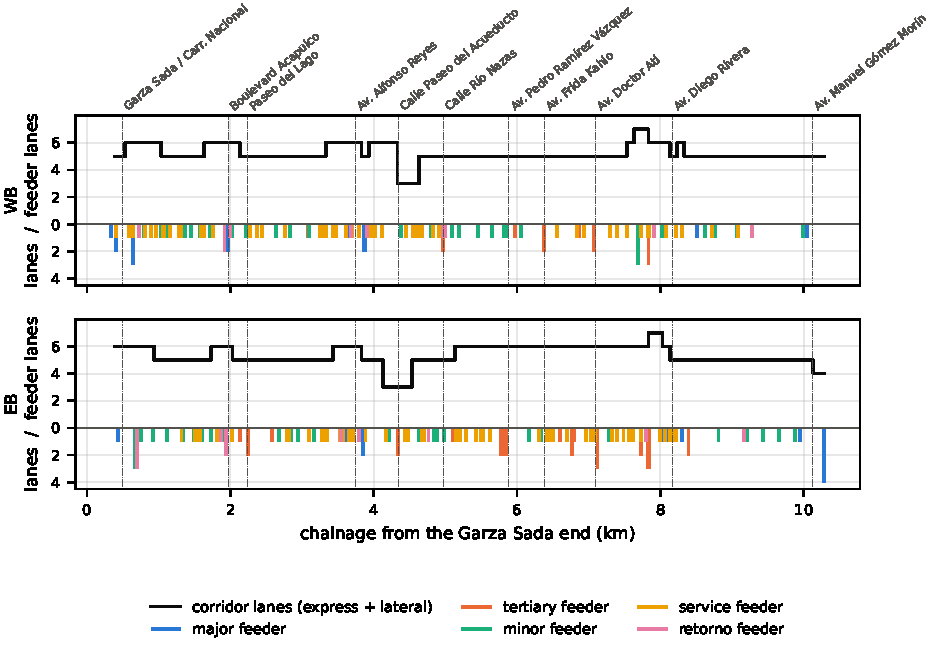
\includegraphics[width=\textwidth]{figures/inventory.pdf}
\caption{Inventory along the corridor, measured from the Garza Sada end
(top: westbound, towards San Pedro; bottom: eastbound). Black: corridor
lanes per direction (express plus frontage). Below the axis: every feeder
approach, with stem length equal to its lanes, coloured by road class.
Dotted lines mark the \InvJunctions\ junctions that split the corridor
into segments. Note the drop to three lanes at 4.4--4.6\,km.}
\label{fig:inventory}
\end{figure*}

\paragraph{Extraction.} We download the street network in 0.01-degree
tiles along the corridor from the OpenStreetMap API (the Overpass mirrors
were saturated on the day). The corridor consists of the \texttt{trunk}
(express) and \texttt{secondary}/\texttt{tertiary} (frontage) ways named
L\'azaro C\'ardenas that lie within 120\,m of the centre line. We assign
each one-way way to a direction by its travel direction along the
chainage. Every other street way that touches a corridor node is a
candidate feeder. One-way tags decide whether it can deliver vehicles
(an approach), receive them (a departure), or both. Chains of unnamed
links that only join the corridor to itself (express--frontage
transfers, U-turns, median crossings) are internal; we found
\InvInternalLinks\ such ways and removed them. A link that does reach the
outside takes the demand class of the most important road it reaches, so
a ramp that only leads to a parking aisle counts as a service access.

\paragraph{What feeds the avenue.} Over \InvLengthKm\,km we find
\InvApproaches\ approaches. \InvServiceApproaches\ of them are
\texttt{service} ways (driveways, plaza and parking entrances), and
\InvNRetorno\ are retornos (U-turns and median crossings that bring
vehicles from the opposite carriageway, \InvLanesRetorno\ lanes; each is
also an exit of the direction it leaves). The other
\InvApproachesNoService\ are streets: \InvNMajor\ major (trunk, primary,
secondary and their links), \InvNTertiary\ tertiary and \InvNMinor\
residential. Together the streets bring \InvFeederLanesNoService\ feeder
lanes (\InvFeederLanes\ including driveways). \InvTerminal\ approaches end
at the corridor (T-junctions, ramps); \InvCrossing\ cross it. The
cross-section is \InvExpressLanes\ express lanes plus two or three
frontage lanes, for a median of \InvMainlineLanes\ lanes per direction
(range \InvMainlineMin--\InvMainlineMax).

The conversation that motivated this project estimated
\LLMAccLo--\LLMAccHi\ accesses, \LLMLanesLo--\LLMLanesHi\ feeder lanes and
\LLMMainLo--\LLMMainHi\ lanes per direction, without giving sources. The
street counts land inside all three ranges. The lane ratio is real: about
\InvLaneRatioNoService:1 without driveways and \InvLaneRatio:1 with them.
The question is whether it means anything.

\paragraph{Data quality.} All corridor ways carry a \texttt{lanes} tag
(\InvCorridorTaggedPct\%). Only \InvTaggedPct\% of the feeder approaches
do; the rest take a class default (one lane per direction for
residential and service, two for tertiary). OpenStreetMap marks only
\InvSignalsOSM\ traffic signals on the corridor, all at Alfonso Reyes.
That is surely incomplete, so we also treat as signalised every frontage
junction fed by a major street or a tertiary street with at least two
lanes. This gives \InvSignalsWB\ signalised cells westbound and
\InvSignalsEB\ eastbound. The model's main bottleneck depends on one
mapped feature, and we test it directly (Section~\ref{sec:results}):
between 4.36 and 4.55\,km the frontage road merges into the express lanes
through a \texttt{secondary\_link} and reappears only after the stretch,
so the corridor narrows from five lanes to three between the Alfonso Reyes
overpass and the bridge over the Canal del Arroyo Seco.

\paragraph{One field estimate.} Alfonso Reyes reaches the corridor with
four lanes from the south. Two of them join L\'azaro C\'ardenas towards
San Pedro (westbound). While Alfonso Reyes has red, only one of them moves,
through a continuous turn; on green both move. An observer on site
estimated 7--10 vehicles per minute on red and 14--18 on green. Weighting
by the model's green share for the cross street gives
\FcWBLo--\FcWBHi\,veh/h for the whole junction (named street and its
unnamed ramps, retornos excluded). The demand model had assumed
\FcWBAssumed\,veh/h there, mostly from a two-lane slip ramp rated as a
major feeder. The count replaces the assumption: the base run uses the
middle of the range, the Monte Carlo draws inside it, and the
continuous-turn lane bypasses the signal. The count records what entered,
so it equals demand only if no queue remains on Alfonso Reyes after the
green; it is an estimate, not a measurement.

\section{Model}
\label{sec:model}

\paragraph{Cells and feeders.} Each direction is a line of 100\,m cells
in travel order. The capacity of cell $i$'s downstream boundary is
\begin{equation}
Q_i = s_0\,\big(\ell^{\mathrm{exp}}_i + \ell^{\mathrm{lat}}_i g_i\big)\,
\big(1 - f\,n^{\mathrm{acc}}_i\big),
\end{equation}
with saturation flow $s_0 = 1900$\,veh/h/lane \cite{hcm2000}, express and
frontage lanes $\ell$, green ratio $g_i$ at signalised cells (\ThG\ at
base), and a friction loss $f$ (\ThFriction\% at base) for each
unsignalised access $n^{\mathrm{acc}}_i$ in the cell. Every approach is a
point queue that discharges at most at its own capacity. That capacity is
$s_0(1-g-0.1)$ per lane at a signal, 1600\,veh/h per lane for a ramp, and
700\,veh/h per lane for a give-way merge. Through traffic enters at the
upstream end (\ThUp\,veh/h at base).

\paragraph{Demand.} An approach delivers
$q = \ell\,r_{\mathrm{class}}\,\tau$\,veh/h: its lanes, times a per-lane
peak rate by class, times the fraction that turns onto the corridor
($\tau = 1$ when the street ends there, \ThTurnCross\ when it crosses).
Base rates are \ThQMajor, \ThQTertiary, \ThQMinor\ and \ThQService\
veh/h/lane for major, tertiary, residential and service. We cannot
measure these, so the Monte Carlo varies each one over a range roughly
twice that wide (log-uniform). Departures attract vehicles by the same
rule. Their split fractions $\beta_i$ are scaled so that the vehicles
leaving by side streets equal those that entered by them, which keeps
corridor flow bounded.

\paragraph{Three levels.} \emph{Closed forms}: each lane group is a
server. We use Erlang C, M/D/1, Kingman \cite{kingman1961heavy} and
Webster \cite{webster1958signal}, and validate them against a
vehicle-level discrete-event simulator. \emph{Tandem model}: the flow at
cell $k$ is $\lambda_k = \min(\lambda_{k-1}, Q_{k-1})(1-\beta_{k-1}) +
a_k$, where $a_k$ is the flow from feeders that join at $k$, and
utilisation is $\rho_k = \lambda_k / Q_k$. \emph{CTM}
\cite{daganzo1994ctm,daganzo1995ctm}: triangular fundamental diagram
(60\,km/h free flow, 20\,km/h backward wave, 150\,veh/km/lane jam
density), $\Delta t = 6$\,s. Feeders merge with Daganzo's priority rule
(priority proportional to lanes). Diverges are partially FIFO: a fraction
$\phi$ of exiting vehicles is held back when the continuing flow is
blocked ($\phi = 1$ is strict FIFO, $\phi=0$ lets exits leave freely;
base \ThFifo). Discharge from a queued cell falls by a capacity drop of
\ThDrop\% \cite{hall1991capacity,chung2007capacity}. Demand follows a
trapezoidal peak over a five-hour horizon: 45\% of peak, rising for 30
minutes to a two-hour plateau, then falling. Total delay is the
vehicle-hours spent in excess of free flow on the corridor plus all
vehicle-hours waiting in feeder queues. An active bottleneck is a cell
boundary with density above critical upstream and below it downstream
\cite{cassidy1999bottlenecks}.

\paragraph{Predictors.} For each segment between junctions we compute,
without simulation: the local lane ratio (feeder lanes entering the
segment over its corridor lanes); the cumulative lane ratio (all feeder
lanes up to the segment over its lanes, the localised ``150 into 6''
argument); feeder lanes alone (cumulative numerator); capacity alone
($1/\min Q$, geometry and signals without demand); and $\max\rho$. The
ground truth is where the CTM places the principal active bottleneck.

\section{Where the queue forms}
\label{sec:results}

\begin{figure}[t]
\centering
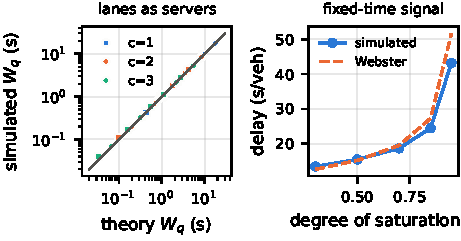
\includegraphics[width=\columnwidth]{figures/validation.pdf}
\caption{Validation. Left: simulated versus theoretical mean wait for
1--3 servers (lanes), Poisson arrivals, exponential (circles) and
deterministic (squares) service, $\rho = 0.3$--$0.9$. Right: delay at a
fixed-time signal (90\,s cycle, $g/C = 0.5$) versus Webster.}
\label{fig:validation}
\end{figure}

\paragraph{Validation.} The discrete-event simulator matches Erlang C,
M/D/1 and Allen--Cunneen with a mean error of \ValErr\% over \ValN\
settings (worst \ValErrMax\%, Allen--Cunneen at light load), and
Webster's signal delay within \ValSigErr\% on average
(Figure~\ref{fig:validation}). Without capacity drop, the CTM's total
delay behind a single lane drop equals the fluid point queue to within
\ValCtmFluidErr\%, as Newell's equivalence requires
\cite{newell1993kinematic}.

\paragraph{The lane count overstates demand by an order of magnitude.}
If every feeder lane discharged at saturation, the \AnaEBSideLanes\
eastbound feeder lanes would deliver about \AnaEBSatVph\,veh/h. Under the
base rates they deliver \AnaEBSideVph\,veh/h, or \AnaEBPerLane\,veh/h per
lane (\AnaEBPerLanePct\% of saturation; westbound \AnaWBPerLane\,veh/h,
\AnaWBPerLanePct\%). Half the approaches are driveways and most of the
rest are one-lane residential streets. Because exits balance the side
inflow, peak corridor flow reaches only \AnaEBPeakFlow\,veh/h eastbound
and \AnaWBPeakFlow\,veh/h westbound.

\begin{figure}[t]
\centering
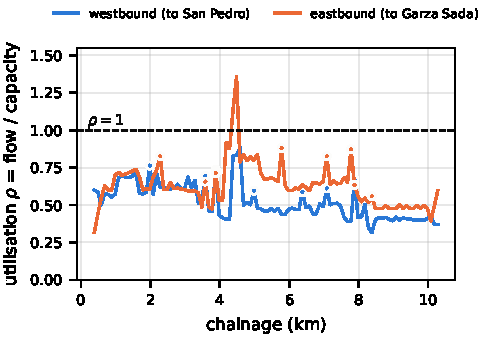
\includegraphics[width=\columnwidth]{figures/utilisation.pdf}
\caption{Steady-state utilisation along the corridor at base parameters;
dots mark signalised cells. Both directions exceed $\rho = 1$ only at the
five-to-three-lane merge near 4.5\,km.}
\label{fig:rho}
\end{figure}

\paragraph{Utilisation picks one place.} Figure~\ref{fig:rho} shows $\rho$
along both directions. It stays below one everywhere except at the merge
between the Alfonso Reyes overpass and the Arroyo Seco bridge, where it
reaches \AnaEBMaxRho\ eastbound. Westbound it peaks at \AnaWBMaxRho\
at the same place. It would be \NcWBMaxRho\ with the assumed demand at
Alfonso Reyes instead of the field estimate. Signals raise $\rho$ locally
but do not push it over one at base parameters.

\begin{figure*}[t]
\centering
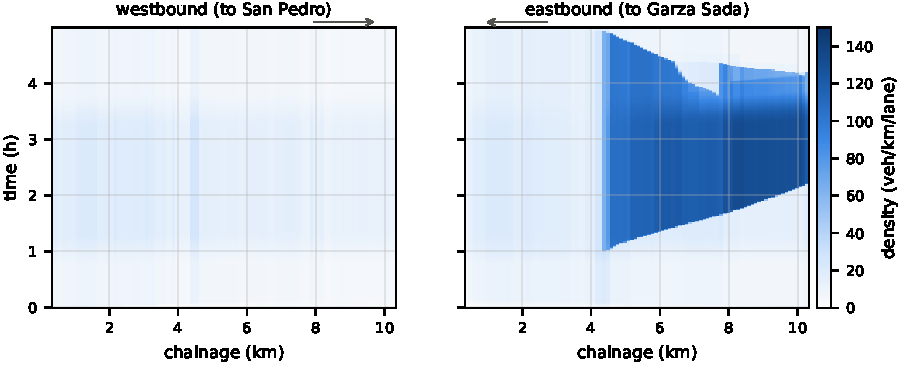
\includegraphics[width=\textwidth]{figures/spacetime.pdf}
\caption{CTM density over time and space at base parameters, both drawn
with chainage increasing to the right (arrows give the travel direction).
Eastbound the queue head stays at the merge (\PeakEBHeadKm\,km) and
backs up across the whole upstream corridor to Gómez Mor\'in; westbound,
with the Alfonso Reyes field estimate, no queue forms.}
\label{fig:spacetime}
\end{figure*}

\paragraph{The peak.} In the CTM (Figure~\ref{fig:spacetime}) the
westbound direction stays free-flowing at base demand. With the assumed
demand at Alfonso Reyes it would queue for \NcWBQueueKm\,km and lose
\NcWBDelay\,veh\,h, so one roadside estimate is enough to remove a
predicted queue. The eastbound queue forms at \PeakEBHeadKm\,km, fills the
\PeakEBQueueKm\,km upstream to Gómez Mor\'in and costs
\PeakEBDelay\,veh\,h (\PeakEBPerVeh\ min per vehicle). A single-bottleneck
fluid queue at the merge would predict \PeakEBFluid\,veh\,h. The
difference comes from the queue reaching feeders and exits upstream. That
is the most uncertain part of the model: with exits that leave freely
($\phi = 0$) eastbound delay is \PeakEBFifoLo\,veh\,h, and with strict
FIFO it is \PeakEBFifoHi. The location of the head does not move.

\begin{figure}[t]
\centering
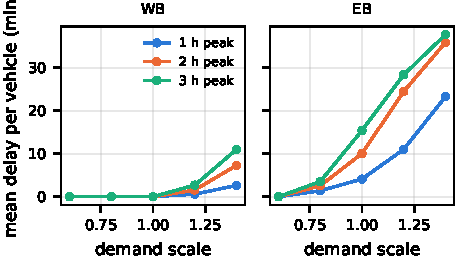
\includegraphics[width=\columnwidth]{figures/demand_grid.pdf}
\caption{Mean delay per vehicle versus a uniform demand scale, for peaks
of 1--3 hours.}
\label{fig:grid}
\end{figure}

\paragraph{Sensitivity to demand.} Scaling all demand
(Figure~\ref{fig:grid}), congestion appears at \GridEBOnset$\times$ base
eastbound and \GridWBOnset$\times$ westbound, where the merge
has about 10\% spare capacity. At
\GridEBTopScale$\times$ with a two-hour peak, mean delay reaches
\GridEBTopPerVeh\ minutes per vehicle eastbound. Delay grows faster than
linearly with peak length, as the fluid model predicts for a queue that
grows throughout the peak.

\begin{figure}[t]
\centering
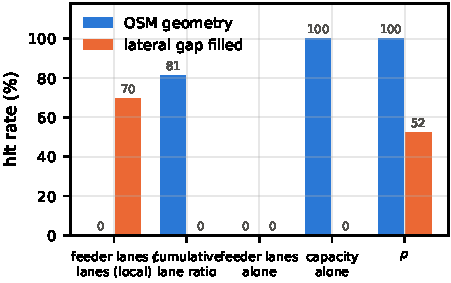
\includegraphics[width=\columnwidth]{figures/predictors.pdf}
\caption{How often each predictor's top segment is the CTM's principal
bottleneck, over \McDraws\ Monte Carlo draws $\times$ 2 directions
(congested runs only), with the OSM geometry and with the frontage gap
filled.}
\label{fig:predictors}
\end{figure}

\paragraph{The test.} Over \McDraws\ Monte Carlo draws of every
assumption (class rates, turn fractions, through demand, green ratio,
friction, $\phi$ and capacity drop), \McCongested\ of \McRuns\
direction-runs congest (Figure~\ref{fig:predictors}). The local lane ratio
picks the right segment in \McHitLR\% of them, and feeder lanes alone in
\McHitFC\%: the segments with the most feeders are not where the queue
starts. The cumulative lane ratio reaches \McHitLRC\%, but only through
its denominator, which drops at the merge. Utilisation reaches
\McHitRho\%. Its maximum also classifies congestion: $\max\rho \ge 1$
agrees with the CTM in \McAcc\% of runs (AUC \McAuc). The lane ratio
cannot do this at all, since it does not change with demand. The
hypothesis survives the falsification rule (falsified: \McFalsified).

There is a caveat, and the Monte Carlo makes it plain: capacity alone
also scores \McHitCap\%. With this geometry, the location is set by the
merge and demand only sets how bad it gets. To see what happens without
it, we fill the frontage gap and rerun. Then only \McGapCongested\ of
\McRuns\ runs congest, westbound congestion disappears at base parameters
($\max\rho = \GapWBMaxRho$; it does not congest at base parameters even with the gap), and eastbound the queue moves to
\GapEBHeadKm\,km. The location now depends on demand, and the ranking changes. Over the
\McGapCongested\ congested runs (all eastbound, mostly one segment), the
local lane ratio finds the bottleneck in \McGapHitLR\% of them,
utilisation in \McGapHitRho\% and capacity alone in \McGapHitCap\%.
Without the merge, the queue starts where many accesses join within a
short stretch. Friction and merge priority in the CTM pull the head there,
while steady-state $\rho$, which treats each cell on its own, points to a
neighbouring segment. So the lane-count argument is not wrong in general.
On this corridor, the lane drop decides the location, and the lane count
cannot see it.

\begin{figure}[t]
\centering
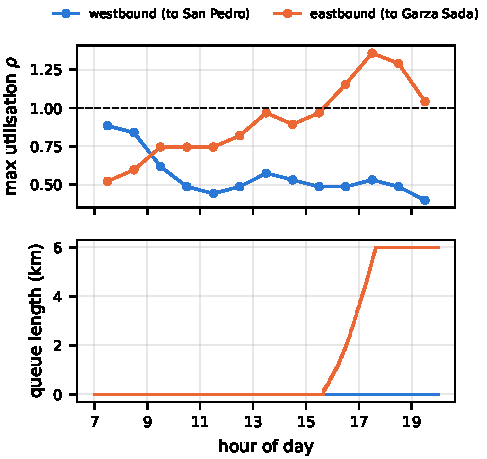
\includegraphics[width=\columnwidth]{figures/daily.pdf}
\caption{A working day, 7:00--20:00, with tidal demand (towards San Pedro
in the morning, towards Garza Sada in the evening). Top: maximum
utilisation along each direction, hour by hour. Bottom: queue length in
the CTM.}
\label{fig:daily}
\end{figure}

\paragraph{A working day.} The tests above use a generic two-hour peak.
Commuting is tidal. We assume that at 7:00 traffic heads south to north,
towards San Pedro and Valle Oriente, and that the evening reverses. The
hourly demand multipliers are set in the configuration
(Figure~\ref{fig:daily}). The maximum capacity at the merge is about
\DayWBCap\,veh/h westbound and \DayEBCap\,veh/h eastbound. With the
Alfonso Reyes estimates, westbound utilisation peaks at \DayWBMaxRho\ at
7:00 and no queue forms; across \DayDraws\ Monte Carlo days, a westbound
queue appears in \DayWBPQueue\%. Eastbound, $\rho$ passes one in the
afternoon. The queue forms at \DayEBStart, reaches \DayEBQueueKm\,km and
\DayEBClears: \DayEBCongH\ congested hours (median \DayEBCongHMed\ over
the Monte Carlo) and \DayEBDelay\,veh\,h within the window. The
observer reports little or no morning queue towards San Pedro, even
though the traffic from Carretera Nacional heads that way. That is the
one qualitative check we have against the field, and the model passes
it. The eastbound afternoon queue has no field check yet.

\section{What would shorten the queue}
\label{sec:interventions}

\begin{figure}[t]
\centering
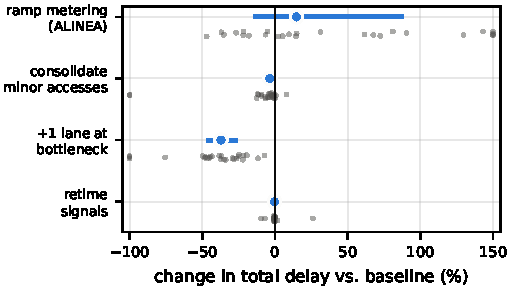
\includegraphics[width=\columnwidth]{figures/interventions.pdf}
\caption{Change in total delay (corridor plus feeder queues) for four
interventions at the CTM's principal bottleneck, over \ItvN\ congested
Monte Carlo direction-runs. Blue: median and interquartile range; grey:
individual runs (clipped at $+150\%$).}
\label{fig:interventions}
\end{figure}

We apply four interventions around the principal bottleneck $b$ in every
congested Monte Carlo run (\ItvN\ direction-runs) and compare total delay
with the same run untreated (Figure~\ref{fig:interventions}).

\paragraph{One more lane over 600\,m at the merge} changes total delay by a
median \ItvLaneMedian\% and helps in \ItvLaneBetter\% of runs. At base parameters
it changes eastbound delay by \ItvLaneBaseEB\%, after which the
next-weakest section becomes the limit. In practice this means extending the frontage road through
the gap, or adding an auxiliary lane on the express side. The model holds
demand fixed, so it omits the extra traffic that new capacity tends to
attract \cite{duranton2011fundamental}.

\paragraph{Ramp metering (ALINEA)} on the four largest feeders within
1.5\,km upstream moves delay rather than removing it: median change
\ItvMetMedian\%, better in \ItvMetBetter\% of runs and worse in
\ItvMetWorse\%. At base parameters eastbound, corridor delay falls from
\ItvBaseEBMain\ to \ItvMetEBMain\,veh\,h while feeder queues grow from
\ItvBaseEBRamp\ to \ItvMetEBRamp. The net gain (\ItvMetBaseEB\%) comes
from avoided capacity drop, and it depends on the drop being large. On an
arterial whose ``ramps'' are residential streets, those waiting vehicles
sit in neighbourhoods.

\paragraph{Consolidating minor accesses} sends residential and service
traffic of each segment to a collector with a single well-designed merge
lane. This removes friction, but it also concentrates the side flow. The
median change is \ItvConMedian\% (better in \ItvConBetter\%, worse in
\ItvConWorse\%).
At base parameters it helps little eastbound (\ItvConBaseEB\%).

\paragraph{Signal retiming} (+0.10 green ratio for the corridor within
1.5\,km upstream and 0.5\,km downstream) barely matters: median
\ItvRetMedian\%. Signals are not where the queue starts, and the green
they gain is taken from cross streets.

\section{Limitations and conclusion}
\label{sec:conclusion}

\paragraph{Limitations.} Apart from one roadside estimate at Alfonso
Reyes, there are no traffic counts in this study. Demand is a parametric model, varied over wide ranges, and every absolute
delay should be read in that light. The conclusions we draw are the ones
that survive the whole Monte Carlo: where the queue forms, and which
predictors find it. The repository accepts field counts
(\texttt{data/field\_counts.csv}, vehicles per hour per approach and
direction, or vehicles per minute on green and red); the Alfonso Reyes
estimate shows how much one count can change: it removed the predicted
westbound queue. Fifteen minutes of video at a few junctions, especially
eastbound, would replace the largest remaining assumptions with data. OpenStreetMap is incomplete in two places
that matter. Signals are under-mapped, so we infer them at major
frontage junctions. The five-to-three-lane merge that dominates the
results is a mapped feature that should be checked on site; if the
frontage road actually continues there, the bottleneck moves, as the
filled-gap experiment shows. The CTM aggregates express and frontage
lanes into one cross-section, applies green ratios as average capacities
rather than cycles, treats each approach as a vertical queue, and gives
every vehicle the same route behaviour. How strongly the queue blocks
exits ($\phi$) changes delay several-fold and is the first thing a field
study should measure. The model has no route choice, so traffic does not
shift to Gómez Mor\'in, Vasconcelos or Garza Sada when L\'azaro C\'ardenas
fills up.

\paragraph{Conclusion.} The lane count behind the popular explanation is
right: about \InvFeederLanesNoService\ street lanes, \InvFeederLanes\
with driveways, into \InvMainlineLanes\ per direction. But it is the
wrong quantity. Feeder lanes carry a few percent of their saturation flow,
and their number does not locate the queue: the local lane ratio found
the bottleneck in \McHitLR\% of congested runs. Utilisation found it in
\McHitRho\% and predicted whether congestion occurs at all. Remove the
lane drop, though, and the lane ratio becomes the better locator
(\McGapHitLR\% against \McGapHitRho\%, in a small sample): where many
accesses join in a short stretch, their friction matters. On this
corridor, at this map, the answer is geometric: a merge from five lanes
to three between Alfonso Reyes and the Arroyo Seco bridge. The
intervention that helps in every run is capacity at that merge, not
fewer driveways or retimed signals. The rule generalises beyond
Monterrey: to find where a corridor jams, compare demand with capacity at
each merge, and look first for the place where lanes disappear.


\FloatBarrier
\bibliographystyle{plain}
\bibliography{references}

\end{document}
